\chapter{Methodology}
\label{sec:methodology}

In Section \ref{sec:research-questions}, we set out to find the cases in which Ask-Elle's normalization does not work as expected. Based on this knowledge, we aim to improve the normalization procedure so it can handle a wider range of programs. We tackle the problem by iterating through the following steps:

\begin{enumerate}
    \item Measure the effectiveness\footnote{Defined as \emph{the amount of clusters and their size, after normalizing the student submissions}. See Section \ref{sec:method-measurement-definitions} for context and more details.} of Ask-Elle's normalization, relative to a set of student programs;
    \item Analyze the set of student programs to reveal normalization shortcomings;
    \item Enhance Ask-Elle's normalization to resolve the discovered shortcomings.
\end{enumerate}

The analysis phase attempts to answer our first research question, while the enhancement phase tackles the second one. The measurement step provides a point of reference.

\section{Measure}
\label{sec:method-measure}

To quantify the initial state of Ask-Elle's normalization and our improvements, we define a series of measurements to be taken on a particular dataset.

\subsection{Dataset}

Our method requires analyzing sets of programs known to be semantically equivalent. To this purpose, we analyze the correct solutions to \emph{Assignment I} of the functional programming course at Universiteit Utrecht in the year 2017/2018.

From the students that participated in the course, there are 111 who submitted a correct solution to the assignment and gave consent for it to be used for research purposes. Students were allowed to submit multiple solutions, but we considered only the final submissions in our research, as each of them is supposed to be the best solution the student was able to write.

% The assignment document \cite{assignment1} provides a high-level description of the task:

% \begin{quote}
%     In this exercise we will read in a database, perform a simple query on it and present the results to the user in an aesthetically pleasing form. Most exercises can be completed by combing functions from the Prelude and the libraries Data.Char, Data.List and Data.Maybe and contain a hint on which functions you could use from these libraries; often a completely different solution, not using these functions, is also possible.
% \end{quote}

In the assignment, the students are asked to implement 8 functions of growing complexity \cite{assignment1}. This translates to 8 Ask-Elle exercises, each one with 111 student solutions. Coincidentally, the functions in the assignment document are labeled as Exercise 1, Exercise 2, etc, up to Exercise 8.

Correctness of the answers was verified through a test suite, which turned out to allow some incorrect programs and thus required minimal clean-up of the data. Table \ref{tb:correct-submissions-per-exercise} shows the amount of correct programs for each exercise, after filtering out those that were wrongly classified as correct.

\begin{table}[H]
\centering
\begin{tabular}{ m{12em} | m{12em} }
    Exercise number & Correct submissions \\
    \hline
    1 & 110 \\
    \hline
    2 & 111 \\
    \hline
    3 & 103 \\
    \hline
    4 & 108 \\
    \hline
    5 & 109 \\
    \hline
    6 & 101 \\
    \hline
    7 & 99 \\
    \hline
    8 & 100
\end{tabular}
\caption{Correct submissions per exercise}
\label{tb:correct-submissions-per-exercise}
\end{table}

\subsection{Measurements}
\label{sec:method-measurement-definitions}

Measurements are done on a per-exercise basis. As a first step, we classify the student submissions into clusters. A \emph{cluster} is \emph{a set of programs that share the same normal form, under a given normalization procedure}. This means that the programs in a cluster are seen as semantically-equivalent by Ask-Elle.

Based on the concept of clusters, we can define the \emph{effectiveness} of normalization as \emph{the amount of clusters and their size, after normalizing the student submissions}. As an example, Figure \ref{fig:method-ex3-clusters} compares the effectiveness for Exercise 3 before and after our research. Without our improvements, there are 51 clusters, where the biggest one contains 29 programs. After our improvements, there are 16 clusters, where the biggest contains 81 programs.

\begin{figure}
\centering
\begin{tabular}{ >{\centering\arraybackslash}m{14em} >{\centering\arraybackslash}m{14em} }
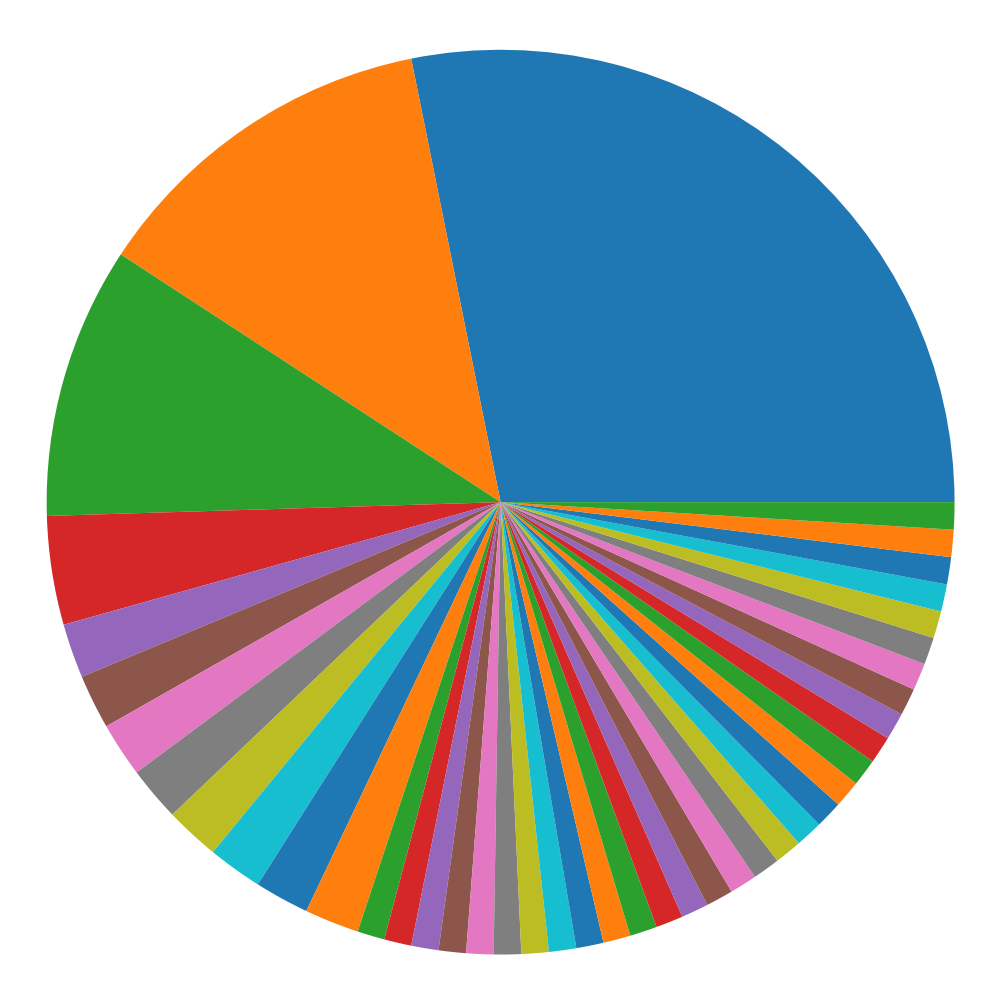
\includegraphics[height=5cm]{graphs/cluster-baseline-3.png}
&
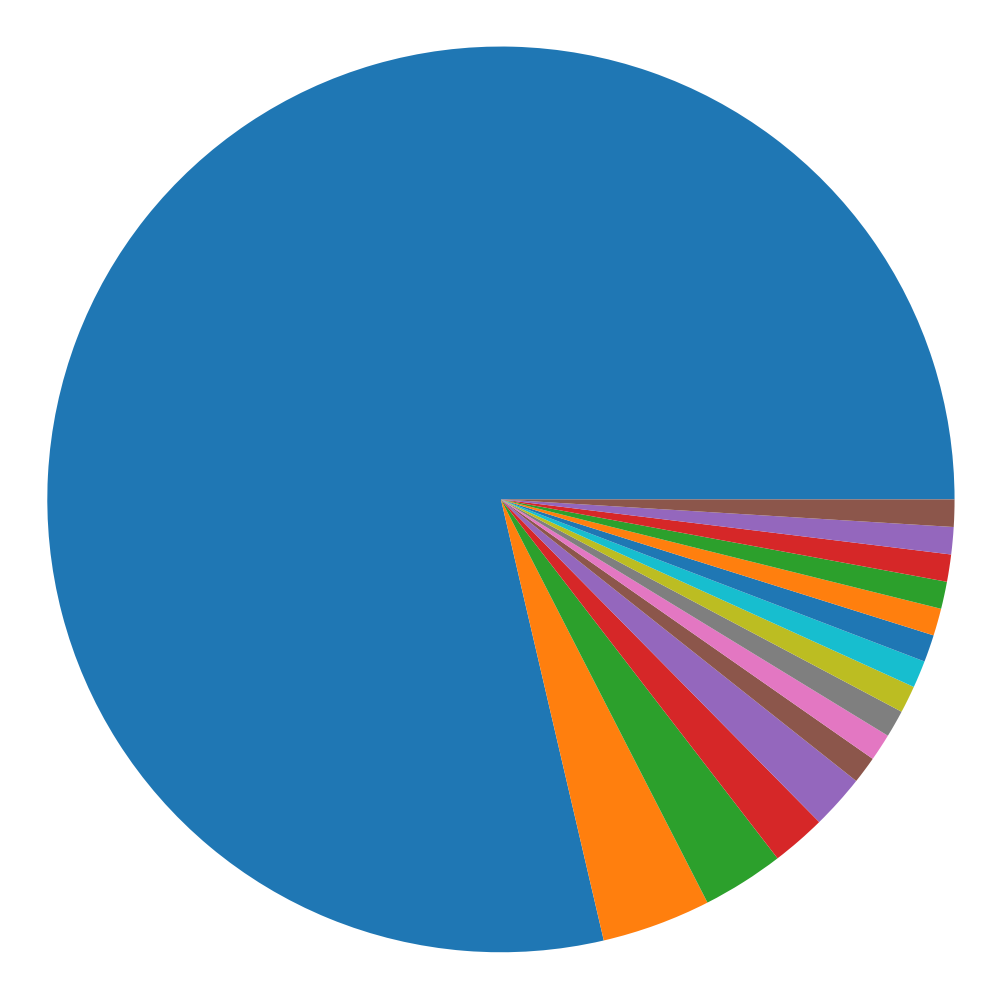
\includegraphics[height=5cm]{graphs/cluster-aggressive-3.png} \\
Before & After
\end{tabular}
\caption{Effectiveness for Exercise 3 before and after improvements}
\label{fig:method-ex3-clusters}
\end{figure}

We say that a given normalization procedure is better or \emph{more effective} than a second one when \emph{it results in a lower amount of clusters for the same exercise}. In the case of Exercise 3, we can say that our improved normalization scheme is more effective than Ask-Elle's original one.

Informally, we can also visualize normalization effectiveness by looking at the percentage of student programs that are recognized by a given amount of model solutions. Again in Exercise 3, Ask-Elle used to recognize 54\% of the submissions based on 4 model solutions. Now, Ask-Elle recognizes 85\% of them based on 3 model solutions.

\section{Analyze}

Identifying shortcomings in the normalization procedure becomes straightforward after classifying the programs into clusters. Informally, our approach consists of repeatedly following the steps below:

\begin{enumerate}
\item Pick one of the biggest clusters;
\item Pick a cluster that is smaller than the current one;
\item Compare the normal forms of both clusters;
\item Identify patterns that should have the same normal form, but do not;
\end{enumerate}

As an example of a limitation we discovered, consider Exercise 1, which consists of implementing the function \texttt{parseTable}. Below we compare the normal forms of two clusters:

\begin{figure}[H]
\centering
\begin{tabular}{ m{13em} | m{13em} }
    Cluster A (73 programs) & Cluster B (13 programs) \\
    \hline
    \begin{minted}{haskell}
parseTable = map words
    \end{minted}
    &
    \begin{minted}{haskell}
parseTable =
    (\x1 -> case x1 of
        x2 -> map words x2
    )
    \end{minted}
\end{tabular}
\caption{Comparing two clusters of Exercise 1}
\label{fig:method-comparing-clusters}
\end{figure}

We can see that both normal forms have the same semantics but are still syntactically different. In this case, it seems reasonable to think of a semantics-preserving tranformation that turns the right-hand side of Cluster B into \haskell{map words}. Figuring out which exact transformation we need is the role of the \emph{enhance} step, explained in the next section.

While the normalization problem identified in the previous example is fairly low-level, we identify higher-level problems too. For instance, Section \ref{sec:analysis-preconditions} explains the interaction between function preconditions and normalization.

\section{Enhance}
\label{sec:method-enhance}

The enhance step bridges the gap between discovering shortcomings and improving Ask-Elle's normalization. Besides adding new transformations to the normalization pipeline, it needs to ensure they are semantics-preserving.

\subsection{Adding a new transformation}

Let us consider the normal forms from Figure \ref{fig:method-comparing-clusters}. We could say that Cluster B is stuck somewhere in the normalization process, instead of arriving at \haskell{map words} as we would expect.

Ask-Elle has an eta-reduction transformation, which could simplify \mintinline{haskell}{\x1 -> map words x1} to \haskell{map words}. However, it fails to work in the case of Cluster B because there is a \haskell{case} expression.

Ask-Elle also has an inlining transformation, which replaces a variable usage by its definition. In the case of Cluster B, it seems sensible that \haskell{x2} could be replaced by \haskell{x1}, thereby getting rid of the \haskell{case}. However, given that \haskell{case} is a very expressive Haskell construct, the inlining transformation does not support it. Instead, it only supports \haskell{let} bindings.

One possible solution is to add a normalization step that, for any \haskell{case} expression consisting of a single alternative with only a var pattern, rewrites it in terms of \haskell{let}. In the case of Cluster B, this transformation would allow the inliner to simplify the code further in a later pass, which opens the door to eta reduction.

\begin{figure}[H]
\centering
\begin{tabular}{ m{8em} | m{8em} }
    Before & After \\
    \hline
    \begin{minted}{haskell}
case e of
    x -> e'
    \end{minted}
    &
    \begin{minted}{haskell}
let x = e
in e'
    \end{minted}
\end{tabular}
\caption{Transforming a case into a let}
\label{fig:method-case-to-let}
\end{figure}

\subsection{Soundness}

We say that a transformation is sound when it is semantics-preserving. That is, for any program, the transformed program is semantically equivalent to the original one.

To increase our confidence in the soundness of the new transformations, we resort to formal proofs and property-based testing.

\paragraph{Formal proofs}

Throughout our research, we added around 60 transformations to Ask-Elle. Formalizing and proving that all of them are semantics-preserving would be a research project of its own. Still, we formalized and proved the soundness property for 31 of them in Coq.

When choosing which transformations to prove we discarded trivial ones (e.g. rewrite rules that are true by definition) and others that were too complex (e.g. anything involving scoped variables, like inlining or dead code removal). Instead, we focused on transformations that can be expressed as rewrite rules in Coq's type system.

As an example, consider a hypothetical cluster of programs in Exercise 1 that has the following normal form:

\begin{figure}[H]
\centering
\begin{minted}{haskell}
parseTable =
    (\xs -> case xs of
        [] -> []
        ys -> map words ys
    )
\end{minted}
\caption{Useless case matching before calling map.}
\label{fig:method-bad-style-map}
\end{figure}

We can prove that removing the \haskell{case} expression preserves the semantics of the program, as shown in the \emph{empty\_base\_case} theorem on Figure \ref{fig:formal-proof-example}. The proof says that calling \haskell{map} inside a \haskell{case}, as in Figure \ref{fig:method-bad-style-map}, has the same semantics as calling it directly. The proof is surprisingly simple using Coq's built-in tactics, as is the case for most of the proofs we constructed. We distinguish two possible cases: \haskell{xs} is empty or it is not. In both cases, beta-reduction results in an equality that is true by reflexivity.

\begin{figure}
\centering
\begin{minted}{coq}
Definition bad_style_map
                {T U} (f : T -> U) (xs : list T)
                : list U :=
    match xs with
    | [] => []
    | ys => map f ys
    end.

Theorem empty_base_case : forall {T U} (f : T -> U) xs,
    bad_style_map f xs = map f xs.
Proof.
    intros. (* Introduce variables f and xs *)
    destruct xs. (* Case split on xs *)
        auto. (* Trivially true when xs = [] *)
        auto. (* Trivially true when xs = y :: ys *)
Qed.
\end{minted}
\caption{Proving the soundness of a transformation.}
\label{fig:formal-proof-example}
\end{figure}

\paragraph{Property-based testing}

The original assignment had a basic test suite that we discovered to be insufficient, since some incorrect student solutions were not flagged as such. Therefore we developed our own test suite, specifying properties that each exercise should satisfy.

By feeding the normalized programs to our test suite, we were able to verify that they still satisfy the properties required by the assignment. This proved to be an effective approach, as it caught a few bugs in the implementation of some transformations.
